%%%%%%%%%%%%%%%%%%%%%%%%%%%%%%%%%%%%%%%%%%%%%%%%%%%%%%%%%%%%%%%%%%%%%%%%%%%%%%%%%%%
%% This project aims to create the UFC template for presentation.                %%
%% author: Maurício Moreira Neto - Doctoral student in Computer Science (MDCC)   %%
%% contacts:                                                                     %%
%%    e-mail: maumneto@ufc.br                                                    %%
%%    linktree: https://linktr.ee/maumneto                                       %%
%%%%%%%%%%%%%%%%%%%%%%%%%%%%%%%%%%%%%%%%%%%%%%%%%%%%%%%%%%%%%%%%%%%%%%%%%%%%%%%%%%%
\documentclass{libs/ufc_format}
% Inserting the preamble file with the packages
%%%%%%%%%%%%%%%%%%%%%%%%%%%%%%%%%%%%%%%%%%%%%%%%%%%%%%%%%%%%%%%%%%%%%
%% This file contains the packages that can be used in the beamer. %%
%%%%%%%%%%%%%%%%%%%%%%%%%%%%%%%%%%%%%%%%%%%%%%%%%%%%%%%%%%%%%%%%%%%%%
% Package to fonts family
\usepackage[T1]{fontenc}
% Package to accentuation
\usepackage[utf8]{inputenc}
% Package to Portuguese language
\usepackage[brazil]{babel}
% Package to Figures
\usepackage{graphicx}
% Package to the colors
\usepackage{color}
% Package to the colors
\usepackage{xcolor}
% Packages to math symbols and expressions
\usepackage{amsfonts, amssymb, amsmath}
% Package to multiple lines and columns in table
\usepackage{multirow, array} 
% Package to create pseudo-code
% For more detail of this package: http://linorg.usp.br/CTAN/macros/latex/contrib/algorithm2e/doc/algorithm2e.pdf
\usepackage{algorithm2e}
% Package to insert code
\usepackage{listings} 
\usepackage{keyval}
% Package to justify text
\usepackage[document]{ragged2e}
% Package to manage the bibliography
\usepackage[backend=biber, style=numeric, sorting=none]{biblatex}
% Package to facilities quotations
\usepackage{csquotes}
% Package to use multicols
\usepackage{multicol}

% Packages added by me
\usepackage{url}
\usepackage{tikz}
%\usepackage{multimedia}
%\usepackage{media9}[playbutton=plain, windowed=1280x720]
% Inserting the references file
\bibliography{references.bib}
\renewcommand*{\bibfont}{\scriptsize}

% Title
\title[ML]{\huge\textbf{Machine Learning}}
% Subtitle
\subtitle{Parte 2}
% Author of the presentation
\author{Evandro J.R. Silva}
% Institute's Name
\institute[Estácio Teresina]{
    % email for contact
    \normalsize{\email{ejrs.profissional@gmail.com}}
    \newline
    % Department Name
    \department{Bacharelado em Ciência da Computação}
    \newline
    % university name
    %\ufc
    \estaciothe
}
% date of the presentation
\date{\today}


%%%%%%%%%%%%%%%%%%%%%%%%%%%%%%%%%%%%%%%%%%%%%%%%%%%%%%%%%%%%%%%%%%%%%%%%%%%%%%%%%%
%% Start Document of the Presentation                                           %%               
%%%%%%%%%%%%%%%%%%%%%%%%%%%%%%%%%%%%%%%%%%%%%%%%%%%%%%%%%%%%%%%%%%%%%%%%%%%%%%%%%%
\begin{document}
% insert the code style
%%%%%%%%%%%%%%%%%%%%%%%%%%%%%%%%%%%%%%%%%%%%%%%%%%%%%%%%%%%%%%%%%%%%%%%%%%%%%%%%%%%
%% This file contains the style of the codes show in slides.                     %%
%% The package used is listings, but it possible to used others.                 %%
%%%%%%%%%%%%%%%%%%%%%%%%%%%%%%%%%%%%%%%%%%%%%%%%%%%%%%%%%%%%%%%%%%%%%%%%%%%%%%%%%%%

% color used in the code style
\definecolor{codegreen}{rgb}{0,0.6,0}
\definecolor{codegray}{rgb}{0.5,0.5,0.5}
\definecolor{codepurple}{rgb}{0.58,0,0.82}
\definecolor{codebackground}{rgb}{0.95,0.95,0.92}

% style of the code!
\lstdefinestyle{codestyle}{
    backgroundcolor=\color{codebackground},   
    commentstyle=\color{codegreen},
    keywordstyle=\color{magenta},
    numberstyle=\tiny\color{codegray},
    stringstyle=\color{codepurple},
    basicstyle=\ttfamily\footnotesize,
    frame=single,
    breakatwhitespace=false,         
    breaklines=true,                 
    captionpos=b,                    
    keepspaces=true,                 
    numbers=left,                    
    numbersep=5pt,                  
    showspaces=false,                
    showstringspaces=false,
    showtabs=false,                  
    tabsize=2,
    title=\lstname 
}

\lstset{style=codestyle}


%% ---------------------------------------------------------------------------
% First frame (with tile, subtitle, ...)
\begin{frame}{}
    \maketitle
\end{frame}

%% ---------------------------------------------------------------------------
% Second frame
\begin{frame}{Sumário}
    \begin{multicols}{2}
        \tableofcontents
    \end{multicols}
\end{frame}

%=============================================================================
% SECTION 1
%=============================================================================
\section{Principais Algoritmos}

\begin{frame}{}
    \centering
    \LARGE
    Principais Algoritmos
\end{frame}

\begin{frame}{Principais Algoritmos}
    \begin{itemize}
        \item<1-10> Aprendizado Supervisionado
            \begin{itemize}
                \item<2,3-6> Classificação
                    \begin{itemize}
                        \item<3-6> Naive Bayes
                        \item<4-6> k-NN
                        \item<5-6> Árvore de Decisão
                        \item<6> Redes Neurais Artificiais
                    \end{itemize}
                \item<2, 7-8> Regressão
                    \begin{itemize}
                        \item<8> Regressão Logística
                    \end{itemize}
            \end{itemize}
        \item<1, 9-10> Aprendizado Não Supervisionado
            \begin{itemize}
                \item<10> k-Means
            \end{itemize}
    \end{itemize}
\end{frame}

%=============================================================================
% SECTION 2
%=============================================================================
\section{Naive Bayes}

\begin{frame}{}
    \centering
    \LARGE
    Aprendizado Supervisionado\\
    \vspace{0.5cm}
    \LARGE
    Classificação\\
    \vspace{0.5cm}
    \Large
    Naive Bayes
\end{frame}

\begin{frame}{Naive Bayes}
    \begin{itemize}
        \justifying
        \item Naive Bayes é um \textbf{modelo de classificação} baseado na \textbf{probabilidade condicional}.
        \item A partir da Teoria da Decisão Bayesiana, podemos calcular, para uma dada observação, qual sua \alert<2>{classe} mais provável.
            \begin{itemize}
                \justifying
                \item<2> Classe ou categoria. Daí vem o termo \textit{classificação}. A partir de um ou mais atributos podemos separar objetos em diferentes classes.
            \end{itemize}
    \end{itemize}
\end{frame}

\begin{frame}{Naive Bayes}
    Lembremos dos peixes:\\
    \begin{figure}
        \centering
        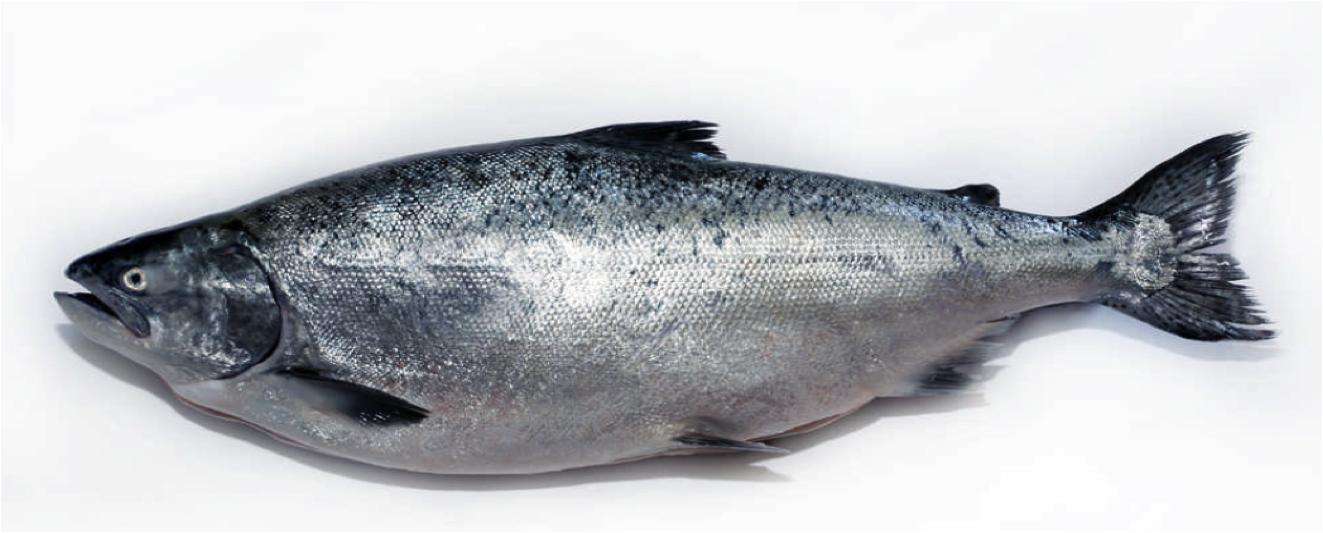
\includegraphics[width=6.5cm]{media/salmon}
        \caption{Salmão}
        \label{fSalmao}
    \end{figure}
    \vspace{-0.5cm}
    \begin{figure}
        \centering
        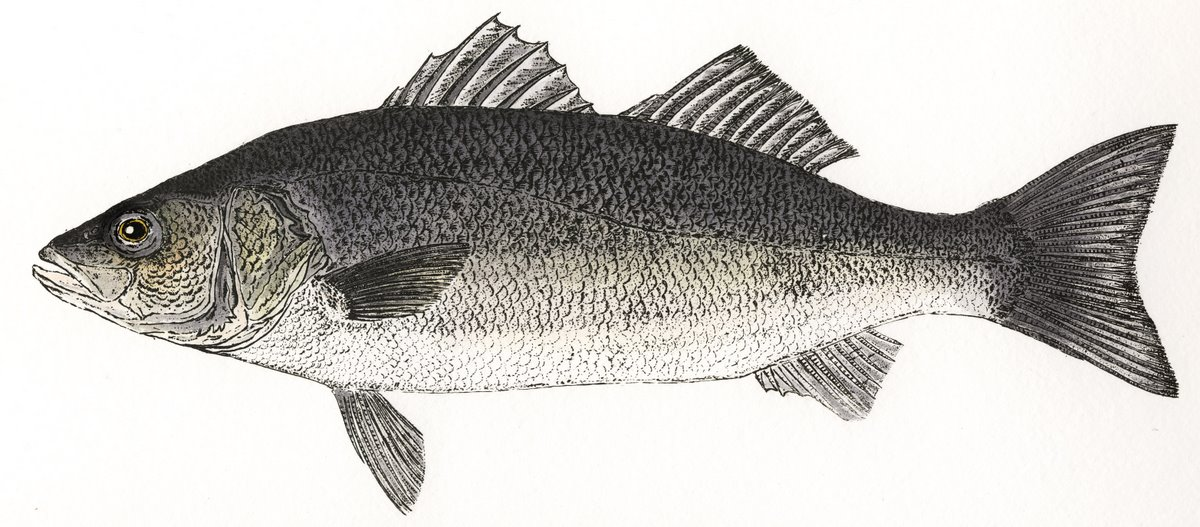
\includegraphics[width=6.5cm]{media/seabass}
        \caption{Robalo}
        \label{fRobalo}
    \end{figure}    
\end{frame}

\begin{frame}{Naive Bayes}
    \begin{itemize}
        \justifying
        \item A tarefa: classificar um peixe como Salmão ou Robalo.
            \begin{itemize}
                \item Classes: $\omega_1 = Robalo$ \hspace{1cm} $\omega_2 = Salm\tilde{a}o$.
            \end{itemize}
        \item<2-> \textit{A priori} não se sabe a qual espécie o peixe pertence.
        \item<3-> O brilho do peixe foi observado.
    \end{itemize}
\end{frame}

\begin{frame}{Naive Bayes}
    \begin{itemize}
        \item Probabilidade \textit{a priori}
            \begin{itemize}
                \justifying
                \item Reflete o quão \textbf{verossímil} é observar uma das duas espécies de peixe.
                \item Se a quantidade de Salmão é \textbf{igual} à quantidade de Robalo, então é igualmente verossímil observar um Salmãou ou um Robalo. Portanto:
                \item<2-> $P(\omega_{1})$: probabilidade \textit{a priori} de se observar um Robalo.
                \item<3-> $P(\omega_{2})$: probabilidade \textit{a priori} de se observar um Salmão.
            \end{itemize}
    \end{itemize}
\end{frame}

\begin{frame}{Naive Bayes}
    \begin{itemize}
        \item Regra de Decisão
            \begin{itemize}
                \item<2-> Informação disponível: \alert<2->{probabilidades \textit{a priori}}.
                \item<3->
                $\hbox{Decisão} = \left\{\begin{array}{rll}
                \omega_{1}, & \hbox{se} & P(\omega_{1}) > P(\omega_{2}) \\
                \omega_{2}, & \hbox{senão} &
                \end{array}\right.$
                \item<4-> Se $P(\omega_{1}) \gg P(\omega_{2})$, a decisão a favor de $\omega_{1}$ estará correta a maior parte do tempo.
				\item<5-> Se $P(\omega_{1}) = P(\omega_{2})$, essa decisão tem apenas 50\% de chance de estar correta.
            \end{itemize}
    \end{itemize}
\end{frame}

\begin{frame}{Naive Bayes}
    \begin{itemize}
        \item Probabilidade Condicional
            \begin{itemize}
                \justifying
                \item<2-> Suponha conhecidas
                    \begin{itemize}
                        \item<3-> As probabilidades \textit{a priori} $P(\omega_{j})$
                        \item<4-> As densidades condicionais $p(x|\omega_{j}), j = 1,2$
                    \end{itemize}
                \item<5-> Suponha que o valor observador do brilho foi $x$.
                \item<6-> Como isso deve influenciar a nossa decisão em relação a que classe o peixe pertence?
                    \begin{itemize}
                        \justifying
                        \item<7> Densidade de probabilidade conjunta: $p(\omega_{j},x)$
                    \end{itemize}
            \end{itemize}
    \end{itemize}
\end{frame}

\begin{frame}{Naive Bayes}
    \begin{itemize}
        \item<1-> Teorema de Bayes\\
        $p(\omega_{j},x) = P(\omega_{j} | x)p(x) = p(x | \omega_{j})P(\omega_{j})$\\
		\hspace{38pt} $\vdots$\\
		$P(\omega_{j} | x) = \dfrac{p(x | \omega_{j})P(\omega_{j})}{p(x)}$
		\item<2-> Em palavras: $posteriori = \dfrac{\hbox{verossimilhança} \times priori}{\hbox{evidência}}$
    \end{itemize}
\end{frame}

\begin{frame}{Naive Bayes}
    \begin{itemize}
        \item \textit{Posteriori}
            \begin{itemize}
                \justifying
                \item<2-> Observando-se $x$ pode-se passar da probabilidade \textit{a priori} $P(\omega_{j})$ para a probabilidade \textit{a posteriori} $P(\omega_{j}|x)$.
                \item<3-> $P(\omega_{j}|x)$: probabilidade da classe ser $\omega_{j}$ dado que observou-se $x$.
            \end{itemize}
        \item<4-> Verossimilhança
            \begin{itemize}
                \justifying
                \item<5-> Indica que a classe $\omega_{j}$ para o qual $p(x|\omega_{j})$ é maior, é mais verossímil ser a verdadeira classe.
            \end{itemize}
        \item<6-> Evidência
            \begin{itemize}
                \item<7> Fator de escala que garante que a soma das probabilidades \textit{a posteriori} é igual a 1.
            \end{itemize}
    \end{itemize}
\end{frame}

\begin{frame}{Naive Bayes}
    \begin{itemize}
        \item Classificador
            \begin{itemize}
                \justifying
                \item A partir dos cálculos probabilísticos uma \alert<2->{regra de decisão} tem de ser escolhida.
                \item<2-> Uma bastante comum é escolher a hipótese mais provável, de forma a minimizar a probabilidade de erro de classificação.
                \item<3-> Essa regra é conhecida como \textit{máximo a posteriori}.
                \item<4-> $\hat{y} = \underset{k \in \{1,...,K\}}{argmax}p(C_{k})\prod\limits^{n}_{i = 1}p(x_{i} | C_{k})$
                    \begin{itemize}
                        \justifying
                        \item<5> $\hat{y}$: classificação/resultado;
                        \item<5> $argmax$: argumento máximo, ou seja, o maior valor;
                        \item<5> $K$: quantidade de classes, ou seja, K classes.
                        \item<5> $C_{k}$: classe k, em que $k=1,...,K$;
                        \item<5> $p(C_{k})$: probabilidade da classe k;
                        \item<5> $p(x_{i} | C_{k})$: probabilidade da observação $x_{i}$ dada a classe k;
                        \item<5> $n$: quantidade de observações.
                    \end{itemize}
            \end{itemize}
    \end{itemize}
\end{frame}

\begin{frame}{Naive Bayes}
    \begin{itemize}
        \item Exemplo
            \begin{itemize}
                \justifying
                \item Usuários costumam avaliar \textit{designs} preliminares de produtos. Anteriormente, 95\% dos produtos de alto sucesso receberam boas notas, 60\% dos produtos de sucesso moderado receberam boas notas, e 10\% dos produtos de baixo sucesso receberam boas notas. Além disso, 40\% dos produtos tiveram alto sucesso, 35\% tiveram sucesso moderado e 25\% tiveram baixo sucesso.
                    \begin{enumerate}[(a)]
                        \justifying
                        \item Qual a probabilidade de um produto ter uma boa nota?
                        \item Se um novo \textit{desing} recebe uma boa nota, qua é a probabilidade de que ele venha a ter um alto sucesso?
                        \item Se um produto não tem uma boa nota, qual é a probabilidade de ele vir a ter um alto sucesso?
                    \end{enumerate}
            \end{itemize}
    \end{itemize}
\end{frame}

\begin{frame}{Naive Bayes}
    \begin{itemize}
        \item Exemplo
            \begin{itemize}
                \item \textbf{A} = Alto sucesso
                \item \textbf{M} = Médio sucesso
                \item \textbf{B} = Baixo sucesso;
                \item \textbf{N} = Nota boa
                \item \textbf{N'} = Nota ruim
            \end{itemize}
    \end{itemize}
    \vspace{0.15cm}
    \centering
    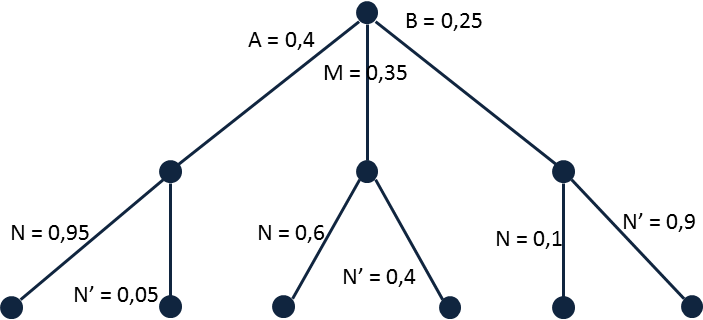
\includegraphics[scale=0.5]{media/questao2}
\end{frame}

\begin{frame}{Naive Bayes}
    \begin{exampleblock}{Resolução}
        \textbf{(a)} Probabilidade de um produto ter uma boa nota\\
        $P(N) = P(N|A)P(A) + P(N|M)P(M) + P(N|B)P(B) = 0,615$\\
        \vspace{0.5cm}
        \textbf{(b)} Probabilidade de ter um alto sucesso se receber nota boa\\
        $P(A|N) = \dfrac{P(N|A)P(A)}{P(N)} = 0,618$\\
        \vspace{0.5cm}
        \textbf{(c)} Probabilidade de ter um alto sucesso se receber nota ruim\\
        $P(A|N') = \dfrac{P(N'|A)P(A)}{P(N')} \rightarrow P(N')?$\\
        $P(N') = P(N'|A)P(A) + P(N'|M)P(M) + P(N'|B)P(B) = 0,385$\\
        $\therefore$\\
        $P(A|N') = 0,052$
    \end{exampleblock}
\end{frame}

%=============================================================================
% SECTION 3
%=============================================================================
\section{k-NN}

\begin{frame}{}
    \centering
    \LARGE
    Aprendizado Supervisionado\\
    \vspace{0.5cm}
    \LARGE
    Classificação\\
    \vspace{0.5cm}
    \Large
    k-NN
\end{frame}

\begin{frame}{k-NN}
    \begin{itemize}
        \justifying
        \item k-NN = k \textit{Nearest Neighbors} ou k Vizinhos Mais Próximos.
        \item A estimação é baseada na probabilidade \textit{a posteriori}.\\
        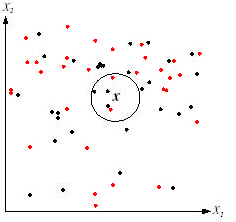
\includegraphics[scale=0.75]{media/knn}
        \item<2-> $P(vermelho) = 2/5 \therefore P(preto) = 3/5$
    \end{itemize}
\end{frame}

\begin{frame}{k-NN}
    \begin{itemize}
        \item k é um número que pode variar\\
        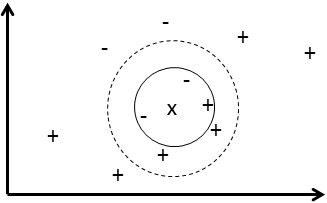
\includegraphics[scale=1]{media/knn_desafio}
    \end{itemize}
\end{frame}

\begin{frame}{k-NN}
    \begin{itemize}
        \justifying
        \item Como \textit{observar} a vizinhança?
            \begin{itemize}
                \justifying
                \item<2-> Distância Euclidiana (mais comum)
                \item<3-> $\hbox{Distância} = \sqrt{\sum\limits^{d}_{i=1}(p_{i} - q_{i})^2}$
                \item<4-> \textbf{Exemplo}: $a_{1}$ = (1, 1); $a_{2}$ = (4, 5)\\
                Distância($a_{1}, a_{2}$) = $\sqrt{(1 - 4)^2 + (1-5)^2}$\\
                Distância($a_{1}, a_{2}$) = $\sqrt{9 + 16}$ = 5
            \end{itemize}
        \item<5> Depois de calcular a distância de um ponto a todos os outros, é possível saber quem são os mais próximos, e suas classes.
    \end{itemize}
\end{frame}

%=============================================================================
% SUBSECTION 4
%=============================================================================
\section{Árvore de Decisão}

\begin{frame}{}
    \centering
    \LARGE
    Aprendizado Supervisionado\\
    \vspace{0.5cm}
    \LARGE
    Classificação\\
    \vspace{0.5cm}
    \Large
    Árvore de Decisão
\end{frame}

\begin{frame}{Árvore de Decisão}
    \begin{itemize}
        \justifying
        \item Segundo Mitchell \cite{m97} \textbf{Árvore de Decisão} é um método para \textbf{aproximação de funções} com \alert<2>{\textbf{valores discretos}}, onde a função aprendida é representada por uma árvore de decisão.
        \item<2> Algoritmos mais recentes permitem a criação de árvores de decisão com valores contínuos.
    \end{itemize}
\end{frame}

\begin{frame}{Árvore de Decisão}
    \begin{itemize}
        \item Representação/Visualização de uma árvore
            \begin{itemize}
                \item Exemplo retirado de \cite{l12}
            \end{itemize}
    \end{itemize}
    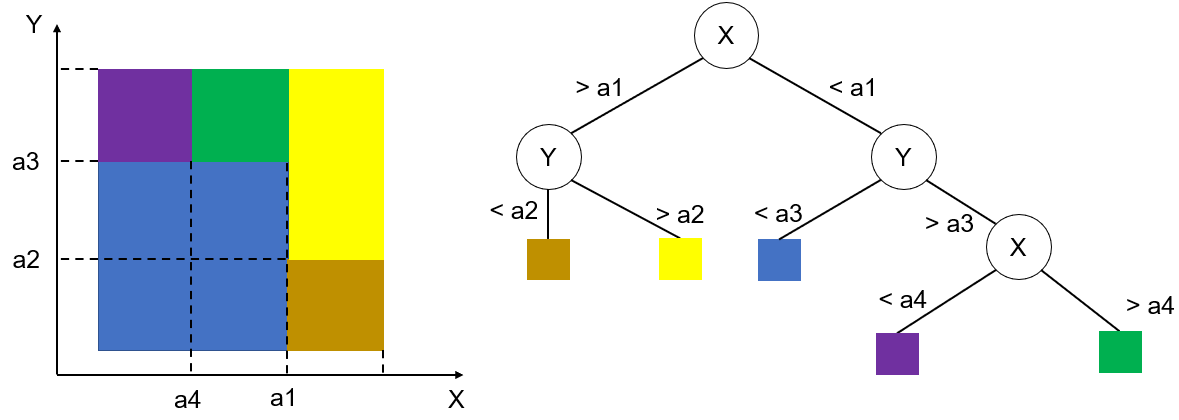
\includegraphics[width=\textwidth]{media/arvore_visual}
\end{frame}

\begin{frame}{Árvore de Decisão}
    \begin{itemize}
        \item Termos técnicos de uma árvore
    \end{itemize}
    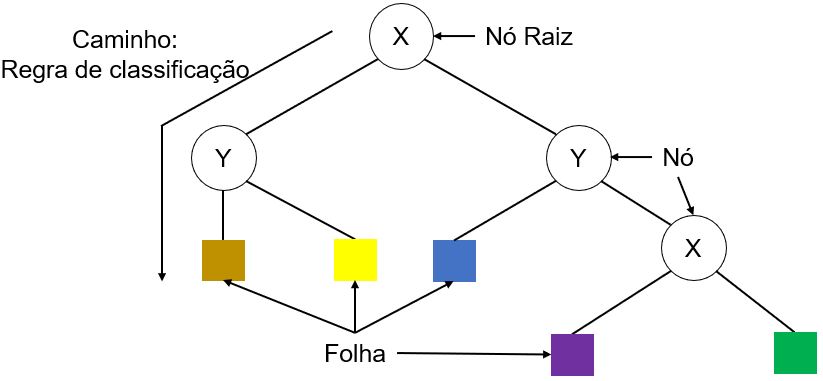
\includegraphics[width=\textwidth]{media/arvore_termos}
\end{frame}

\begin{frame}{Árvore de Decisão}
    \begin{itemize}
        \item<1-9> Como construir?
        \item<2-8> Ideia base:
            \begin{enumerate}
                \justifying
                \item<3-8> Escolher um atributo;
                \item<4-8> Estender a árvore adicionando um ramo para cada valor do atributo;
                \item<5-8> Passar os exemplos para as folhas (tendo em conta o valor do atributo escolhido);
                \item<6-8> Para cada folha
                    \begin{itemize}
                        \justifying
                        \item<7-8> Se todos os exemplos são da mesma classe, associar essa classe à folha;
                        \item<8> Senão, repetir os passos 1 a 4.
                    \end{itemize}
            \end{enumerate}
        \item<9-> Como escolher o melhor atributo?
            \begin{itemize}
                \justifying
                \item<10-> Um atributo deve ser o mais discriminante possível!
                \item<11-> Uma divisão, a partir de um atributo, que mantem as proporções de classes nas folhas é inútil.
                \item<12-> Já uma divisão que tem como resultado todos os exemplos de uma folha sendo da mesma classe, tem utilidade máxima.
            \end{itemize}
    \end{itemize}
\end{frame}

\begin{frame}{Árvore de Decisão}
    \begin{itemize}
        \item Algoritmo ID3 (\textit{Inductive Decision Tree} \cite{q86})
            \begin{itemize}
                \justifying
                \item Para escolher o melhor atributo, é feito um cálculo estatístico conhecido como \textbf{ganho de informação}.
                \item<2-> $G(S,A) \equiv Entropia(S) - \sum\limits_{v \in \alert<3>{Valores(A)}}\dfrac{|\alert<4>{S_{v}}|}{|S|}Entropia(S_{v})$
                    \begin{itemize}
                        \justifying
                        \item<3-4> Conjunto de todos os possíveis valores para o atributo A;
                        \item<4> Subconjunto de $S$ para o qual o atributo A tem valor $v$;
                    \end{itemize}
                \item<5-> Para entender essa fórmula, vamos ver seus elementos.
                \item<6> Começando pela Entropia.
            \end{itemize}
    \end{itemize}
\end{frame}

\begin{frame}{Árvore de Decisão}
    \begin{itemize}
        \justifying
        \item A Entropia é uma medida que caracteriza a pureza ou impureza de um conjunto arbitrário de exemplos \cite{m97}.
        \item<2-> Seja um conjunto $S$ contendo duas classes, uma positiva ($p_{\oplus} =$ proporção de exemplos positivos) e uma negativa ($p_{\ominus} =$ proporção de exemplos negativos).
        \item<3-> A entropia de S é:\\
        $Entropia(S) \equiv -p_{\oplus}log_{2}p_{\oplus} - p_{\ominus}log_{2}p_{\ominus}$\\
        ou\\
        $Entropia(S) \equiv \sum\limits_{i=1}^{c} - p^{}_{i}log^{}_{2}p^{}_{i}$
    \end{itemize}
\end{frame}

\begin{frame}{Árvore de Decisão}
    \begin{exampleblock}{Exemplo}
        \justifying
        S = 14 exemplos ... [9+, 5-]\\
        \uncover<2->{Entropia(S) = Entropia([9+, 5-])}\\
        \uncover<3->{= $-(9/14)log_{2}(9/14) - (5/14)log_{2}(5/14) = 0,940$}
    \end{exampleblock}
\end{frame}

\begin{frame}{Árvore de Decisão}
    \begin{itemize}
        \item Exemplo ilustrativo
    \end{itemize}
    \begin{table}[]
        \centering
        \small
        \begin{tabular}{l c c c c c}
        \hline
            \textbf{Dia}    &  \textbf{Tempo}  &   \textbf{Temperatura}    &   \textbf{Umidade}    &   \textbf{Vento}   & \textbf{Jogar}\\
            \hline
            D1  &   Ensolarado  &   Quente  &   Alta    &   Fraco   &   \alert<3>{Não}\\
            D2  &   Ensolarado  &   Quente  &   Alta    &   Forte   &   \alert<3>{Não}\\
            D3  &   Nublado     &   Quente  &   Alta    &   Fraco   &   \alert<2>{Sim}\\
            D4  &   Chuvoso     &   Média   &   Alta    &   Fraco   &   \alert<2>{Sim}\\
            D5  &   Chuvoso     &   Frio    &   Normal  &   Fraco   &   \alert<2>{Sim}\\
            D6  &   Chuvoso     &   Frio    &   Normal  &   Forte   &   \alert<3>{Não}\\
            D7  &   Nublado     &   Frio    &   Normal  &   Forte   &   \alert<2>{Sim}\\
            D8  &   Ensolarado  &   Média   &   Alta    &   Fraco   &   \alert<3>{Não}\\
            D9  &   Ensolarado  &   Frio    &   Normal  &   Fraco   &   \alert<2>{Sim}\\
            D10 &   Chuvoso     &   Média   &   Normal  &   Fraco   &   \alert<2>{Sim}\\
            D11 &   Ensolarado  &   Média   &   Normal  &   Forte   &   \alert<2>{Sim}\\
            D12 &   Nublado     &   Média   &   Alta    &   Forte   &   \alert<2>{Sim}\\
            D13 &   Nublado     &   Quente  &   Normal  &   Fraco   &   \alert<2>{Sim}\\
            D14 &   Chuvoso     &   Média   &   Alta    &   Forte   &   \alert<3>{Não}\\
            \hline
        \end{tabular}
        \caption{Exemplos de treino para a decisão de jogar}
        \label{t1}
    \end{table}
\end{frame}

\begin{frame}{Árvore de Decisão}
    \begin{exampleblock}{Ganho de Informação}
        \justifying
        $S = [9+, 5-] \rightarrow Entropia = 0,940$\\
        \uncover<2->{Atributo: Tempo = [Ensolarado, Nublado, Chuvoso]}\\
        \uncover<3->{$S_{Ensolarado} = [2+, 3-]$;}\\
        \uncover<4->{$S_{Nublado} = [4+, 0-]$;}\\
        \uncover<5->{$S_{Chuvoso} = [3+, 2-]$;}\\
        \vspace{0.5cm}
        \uncover<6->{$G(S,A) \equiv Entropia(S) - \sum\limits_{v \in Valores(A)}\dfrac{|S_{v}|}{|S|}Entropia(S_{v})$}\\
        \vspace{0.2cm}
        \uncover<7->{$G(S,Tempo) \equiv 0,940 - (5/14)Entropia(S_{Ensolarado})$\\ 
        $\hspace{2cm} - (4/14)Entropia(S_{Nublado}) - (5/14)Entropia(S_{Chuvoso})$}\\
        \vspace{0.2cm}
        \uncover<8->{$G(S,Tempo) \equiv 0,940 - (5/14)0,971 - (4/14)0 - (5/14)0,971$}\\
        \uncover<9->{$G(S,Tempo) \equiv 0,940 - 0,347 - 0 - 0,347$}\\
        \uncover<10>{$G(S,Tempo) \equiv 0,246$}
    \end{exampleblock}
\end{frame}

\begin{frame}{Árvore de Decisão}
    \begin{exampleblock}{Ganho de Informação}
        \justifying
        $Ganho(S, Tempo) = 0,246$\\
        $Ganho(S, Temperatura) = 0,029$\\
        $Ganho(S, Umidade) = 0,151$\\
        $Ganho(S, Vento) = 0,048$\\
        \centering
        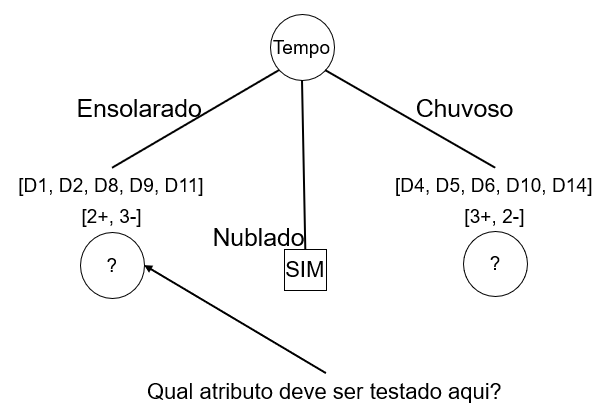
\includegraphics[scale=0.4]{media/arvore_exemplo}
    \end{exampleblock}
\end{frame}

\begin{frame}{Árvore de Decisão}
    \begin{exampleblock}{Próximo Atributo}
        \justifying
        $S_{Ensolarado} =$ [D1, D2, D8, D9, D11]\\
        \hspace{0.5cm}$Ganho(S_{Ensolarado}, Umidade) = 0,970 - (3/5)0 - (2/5)0 = 0,970$\\
        \vspace{0.2cm}
        \hspace{0.5cm}$Ganho(S_{Ensolarado}, Temperatura) = 0,970 - (2/5)0 - (2/5)1$\\
        \hspace{6cm}$- (1/5)0 = 0,570$\\
        \vspace{0.2cm}
        \hspace{0.5cm}$Ganho(S_{Ensolarado}, Vento) = 0,970 - (2/5)1 - (3/5)0,918 = 0,019$\\
    \end{exampleblock}
\end{frame}


%\begin{frame}{Classificação}
%    Agora é com vocês:\\
%    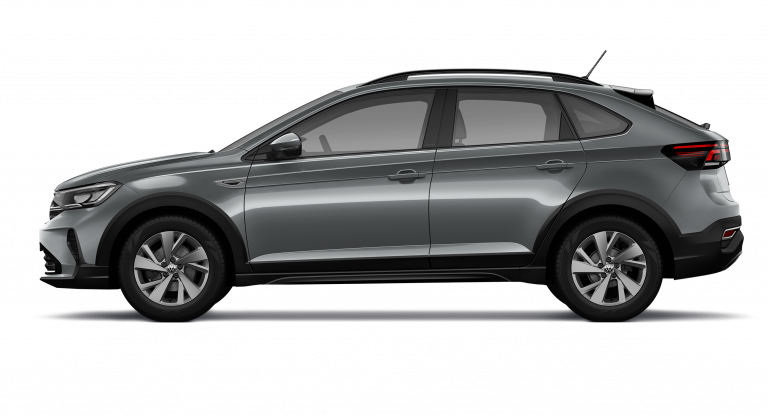
\includegraphics[width=0.5\textwidth, height=0.4\textheight]{media/carro}
%    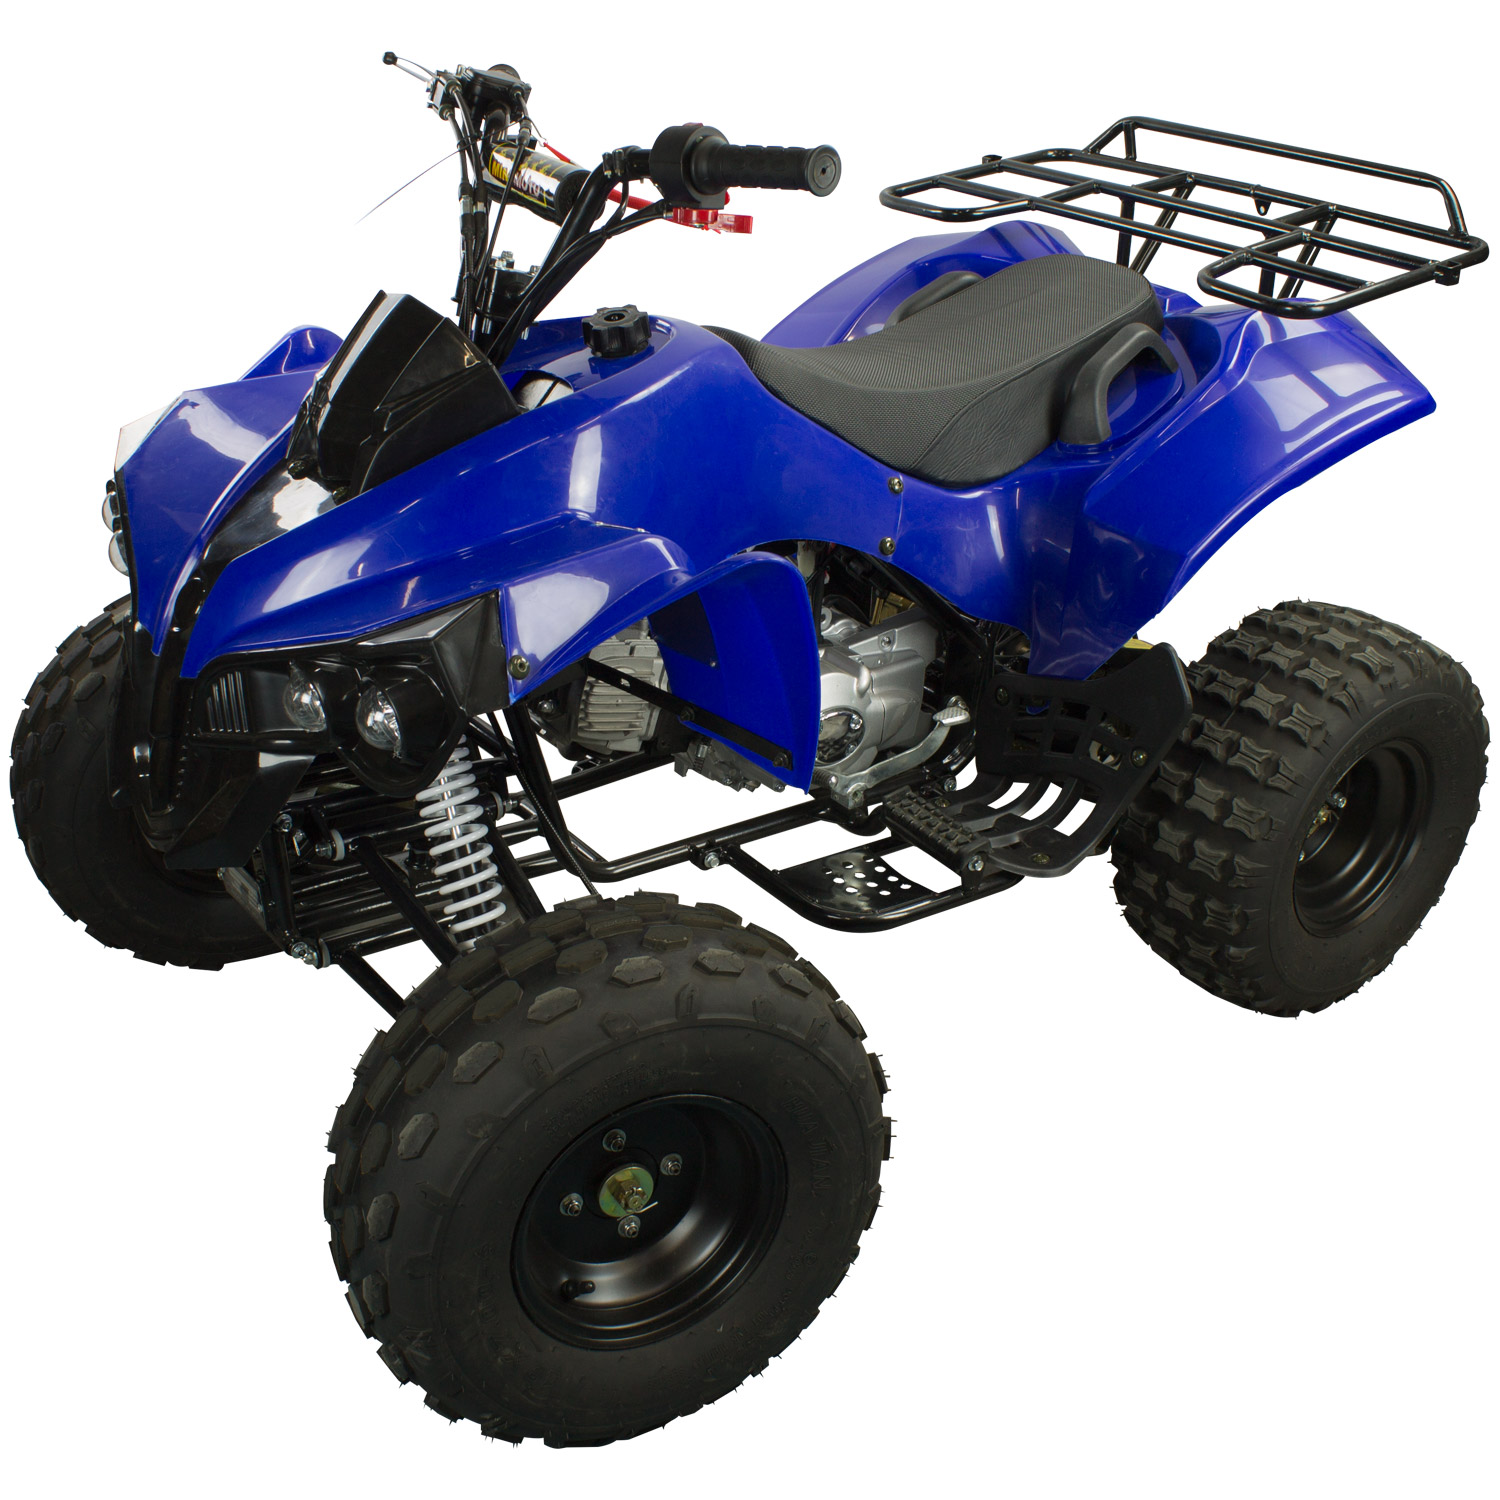
\includegraphics[width=0.5\textwidth, height=0.4\textheight]{media/quadriciclo}\\
%    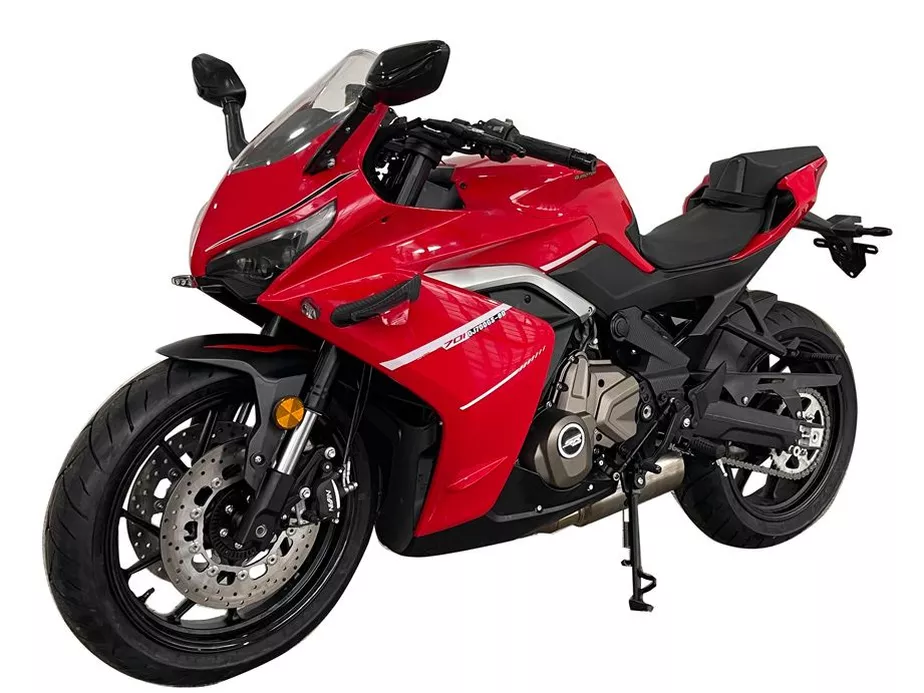
\includegraphics[width=0.5\textwidth, height=0.4\textheight]{media/moto}
%    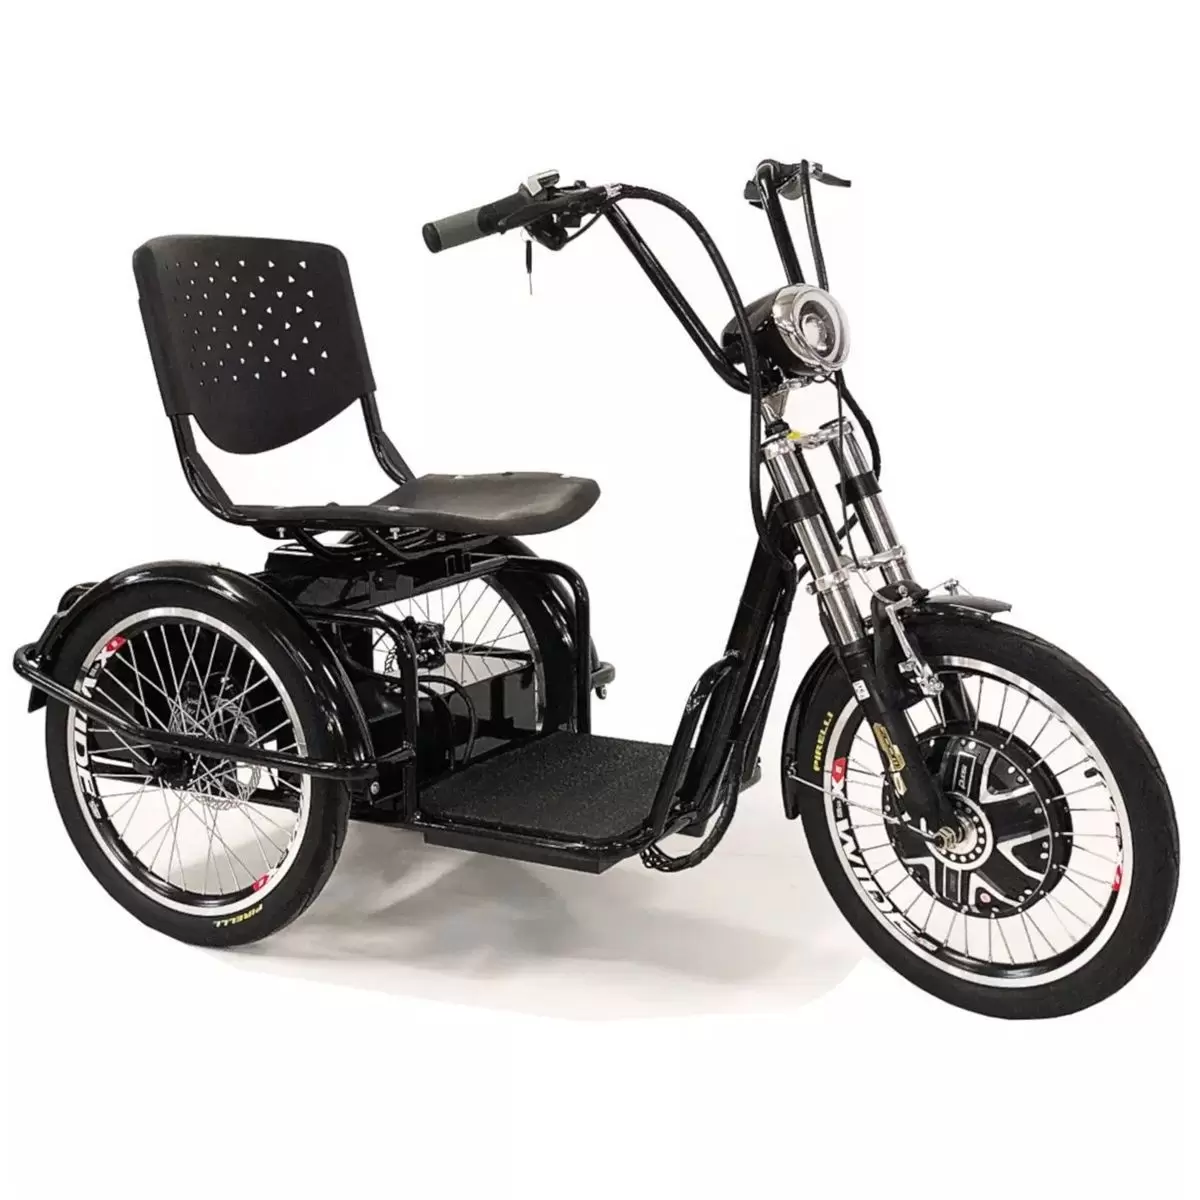
\includegraphics[width=0.5\textwidth, height=0.4\textheight]{media/triciclo}
%\end{frame}

%\item Listar os principais algoritmos, de acordo com as aulas que dei, e com a página de machine learning da wikipedia.
%\item Copiar aulas 2, 3, 4 e 5


%=============================================================================
% SECTION REFERENCES
%=============================================================================
\begin{frame}[allowframebreaks]{Referências}
    \scriptsize
    \printbibliography
\end{frame}

\end{document}













%% ---------------------------------------------------------------------------
% This presentation is separated by sections and subsections
%\section{Seção I}
%\begin{frame}{Explicações}
%    % itemize
%    Este é um template que pode ser utilizado para:
%    \begin{itemize}
%        \item Apresentação de Trabalhos Acadêmicos
%        \item Apresentação de Disciplinas
%        \item Apresentações de Teses e Dissertações
%    \end{itemize}
%
%    \vspace{0.4cm} % vertical space
%    
%    % enumeration
%    Para utilizar este template corretamente é importante que:
%    \begin{enumerate}
%        \item Tenha conhecimento mínimo sobre LaTeX
%        \item Ler os comentários no template (explicações)
%        \item Ler o README.md (documentação)
%    \end{enumerate}
%
%    \vspace{0.2cm}

%    \example{Este é um texto de exemplo!} \emph{Texto de Ênfase!}
%\end{frame}

%% ---------------------------------------------------------------------------
%\subsection{Subseção I}
%\begin{frame}{Criando Blocos}
%    % Blocks styles
%    \begin{block}{Bloco Padrão}
%        Texto do corpo do bloco.
%    \end{block}

%    \begin{alertblock}{Bloco de Alerta}
%        Texto do corpo do bloco.
%    \end{alertblock}
%
%    \begin{exampleblock}{Bloco de Exemplo}
%        Texto do corpo do bloco.
%    \end{exampleblock}   
%\end{frame}

%% ---------------------------------------------------------------------------
%\subsection{Subseção II}
%\begin{frame}{Criando Caixas}
%    \successbox{testando o success box}
%
%    \pause
%
%    \alertbox{testando o alert box}
%
%    \pause
%
%    \simplebox{testando o simple box}
%\end{frame}

%% ---------------------------------------------------------------------------
%\subsection{Subseção III}
%\begin{frame}{Criando Algoritmos (Pseudocódigo)}
%    \begin{algorithm}[H]
%        \SetAlgoLined
%        \LinesNumbered
%        \SetKwInOut{Input}{input}
%        \SetKwInOut{Output}{output}
%        \Input{x: float, y: float}
%        \Output{r: float}
%        \While{True}{
%          r = x + y\;
%          \eIf{r >= 30}{
%           ``O valor de $r$ é maior ou iqual a 10.''\;
%           break\;
%           }{
%           ``O valor de $r$ = '', r\;
%          }
%         } 
%         \caption{Algorithm Example}
%    \end{algorithm}
%\end{frame}

%% ---------------------------------------------------------------------------

%\begin{frame}{Inserindo Algoritmos}
%    \lstset{language=Python}
%    \lstinputlisting[language=Python]{code/main.py}
%\end{frame}

%% ---------------------------------------------------------------------------
%\begin{frame}{Inserindo Algoritmos}
%    \lstinputlisting[language=C]{code/source.c}
%\end{frame}

%% ---------------------------------------------------------------------------
%\begin{frame}{Inserindo Algoritmos}
%    \lstinputlisting[language=Java]{code/helloworld.java}
%\end{frame}

%% ---------------------------------------------------------------------------
%\begin{frame}{Inserindo Algoritmos}
%    \lstinputlisting[language=HTML]{code/index.html}
%\end{frame}

%% ---------------------------------------------------------------------------
% This frame show an example to insert multicolumns
%\section{Multicolunas}
%\begin{frame}{Seção II - Multicolunas}
%    \begin{columns}{}
%        \begin{column}{0.5\textwidth}
%            \justify
%            É possível colocar mais de uma coluna utilizando os comandos de $\backslash$begin\{column\}\{\} e $\backslash$end\{column\}
%        \end{column}
%        \begin{column}{0.5\textwidth}
%            \justify
%            Porém, o espaçamento deve ser proporcional entre as colunas para que estas colunas não entrem em coflito. O espaçamento é dado pelo segundo argumento do $\backslash$begin.
%        \end{column}
%    \end{columns}    
%\end{frame}

%% ---------------------------------------------------------------------------
% This frame show an example to insert figures
%\section{Imagens}
%\begin{frame}{Seção III - Figures}
%    \begin{figure}
%        \centering
%        \caption{Emblema da UFC.}
%        
\includegraphics[scale=0.3]{libs/emblemufc.pdf}
%        \source{Obtido pelo site oficial da UFC \cite{siteufc} \cite{einstein}}
%        \label{fig:ufc_emblem}
%    \end{figure}
%\end{frame}

%% ---------------------------------------------------------------------------
% Reference frames
%\begin{frame}[allowframebreaks]
%    \frametitle{Referências}
%    \printbibliography
%\end{frame}

%% ---------------------------------------------------------------------------
% Final frame
%\begin{frame}{}
%    \centering
%    \huge{\textbf{\example{Obrigado(a) pela Atenção!}}}
%    
%    \vspace{1cm}
%    
%    \Large{\textbf{Contato:}}
%    \newline
%    \vspace*{0.5cm}
%    \large{\email{usuario@dominio}}
%\end{frame}